%%% mode: latex
%%% TeX-master: t
%%% End:

\chapter{绪论}
\label{cha:intro}

\section{研究背景与意义}\label{sec:general intro}
作为互联网信息时代解决信息过载问题的重要工具之一,推荐系统通过分析用户的交互数据和历史行为信息,可以提供相关性、多样性和新颖性的内容选择,能够帮助用户快速准确地找到感兴趣的信息,辅助用户做出更明智的决策。在互联网飞速发展的信息时代,推荐系统在电商、社交媒体、新闻阅读等领域发挥着重要的作用,逐步主导了人们的信息发现过程。因此,推荐算法具有重大研究意义和广阔的应用前景\cite{Steffen:2009:UAI,Ai:2018:SIGIR,Ding:2020:NIPS}。

面向隐式反馈数据的学习排序(Learning-to-Rank)算法根植于对比学习的范式。其中,最广泛使用的成对学习是具有单个负例的对比学习的特例。在完全监督下,对比学习在推荐任务中有很大的优势,主要体现在以下几点:(1)互信息优化:通过
对比语义上相似(正样本)和不相似(负样本)的样本对,拉近锚点与正例的距离,推远锚点与负例的距离,实现对变量互信息的优化。(2)避免过拟合:对比损失激励编码器编码不同样本的差异特征,免于对样本进行像素级信息重构,从而有效的避免了过拟合。(3)排序导向:通过优化成对损失或对比损失,实现了对排序指标AUC和NDCG的优化\footnote{如不考虑正则化项,成对损失函数BPR与AUC指标定义相同,不同之处在于BPR把AUC指标中不可微的$0-1$损失$\ell_{0-1}(\cdot)$替换成了可微的替代损失$\log\sigma(\cdot)$\cite{Steffen:2009:UAI}。}。此外,对比学习在计算机视觉、自然语言处理和信息检索领域取得了巨大的成功,在分类、回归、排序等任务表现出了出色的泛化性能。

受限于推荐系统的场景特征,获取准确的正负样本标签用于对比学习是不实际且昂贵的。传统的有监督学习在推荐中遇到了严重的瓶颈:它不仅严重依赖昂贵的手动标注,而且还面临泛化误差、虚假相关性和对抗性攻击等问题。目前许多最先进的模型都通过对输入数据进行某种变换或处理来创建“伪标签”。通用的做法是将某个用户已交互的物品被标记为正样本,未交互的物品被标记为负样本\cite{Steffen:2009:UAI,Jingtao:2019:IJCAI,Xiangnan:2020:SIGIR,Wang:2019:SIGIR}。类似地,在计算机视觉中,某个样本的增强被标记为正样本,其他样本被标记为负样本\cite{Oord:2018:arxiv,Chen:2020:ICML,He:2020:CVPR,BYOL:2020:NIPS}。

基于自监督技术创建的伪标签,一方面摆脱了对密集人工标注数据集的依赖,使得从海量无监督数据中训练模型成为可能。但另一方面,隐式反馈数据通常是正例-未标注(Positive-Unlabeled, PU)的形式,且正例中包含噪声,如代购、误触等。根据隐式反馈数据交互的有无创建的正负样本标签,不仅导致了伪正例和伪负例的问题,还使得自监督对比学习设置下的优化目标偏离了原始的优化目标,对准确地学习样本的特征表示提出了严峻挑战。如何从弱监督的用户行为数据中学到良好的用户、物品特征表示,是对比学习基础理论的需要,也是提升个性化推荐系统准确性的现实需求。


\section{国内外研究现状}
\label{sec:requirement}
对样本的度量方式主要有两种:一是对样本进行逐个度量,例如个体身高,体重,等。二是在很多高自由度场景中,由于:(1)单个样本的绝对值度量不容易获取;(2)有些度量体现相互关系,只能以成对方式体现;(3)特定场景中更关注相对值的大小而非绝对值的大小,导致了另外一种主要的度量方式出现:成对度量(pairwise measurement)。 例如方案$i$比方案$j$好,用户购买了$i$但是没有购买$j$。成对度量广泛存在于描述客观世界的数据中,度量的方式主要有:(i)成对比较,体现的是强弱关系;(ii)成对关系,例如网页a的超链接指向网页b,体现了相互依存和作用的关系。成对度量提供了从相互关系描述、分析、挖掘事物的视角,相比于逐个度量的方式,突出了数据内部的结构信息,能够更好地描摹客观世界存在的真实形态。

由于用户很少显式地表达对物品的偏好,通常能收集到的数据是一种隐式反馈数据,如点击,购买,浏览等行为数据。贝叶斯个性化排序 (Bayesian Personalized Ranking, BPR)\cite{Steffen:2009:UAI}率先将隐式反馈数据转化为成对比较(Pairwise Comparision)。具体而言,对于某个用户(锚点),观测到的交互物品$i$被标记为正例,无交互的物品$j$被标记为负例,相应的正负例构成一个成对比较实例,意为用户对正例的偏好强于负例。基于构建的成对比较,BPR使用Bradley-Terry模型\cite{Bradley:1952:Biometrika,Luce:2005:JASA}建模成对比较的似然,并通过极大似然估计学习潜在的用户表示和物品表示,从而以为每个用户预测个性化排序。BPR通过将评分预测任务转化为排序预测任务,解决了交互数据无偏好值的问题。由于BPR直接针对排序目标AUC指标进行优化,逐渐主导了从隐式反馈数据中学习排序的任务\cite{Weike:2013:IJCAI,Yu:2018:CIKM,Xiaoye:2011:MathProg,Xuejiao:2020:ASC,Qiu:2018:IS,Zhao:2019:FGCS}。

这种从成对比较中学习排序的方法,在推荐中被称作成对学习。成对学习拥有广泛的应用领域\cite{Bradley:1952:Biometrika,Maystre:2017:ICML,Yang:2020:IS},如决策制定\cite{McFadden:1974:FE}、网络搜索\cite{Dwork:2001:WWW}、信息检索\cite{Ai:2018:SIGIR}、偏好加总\cite{Arrow:2012}等。值得指出的是,BPR损失与噪声对比估计\cite{Gutmann:2010:ICAIS,gutmann:2012:JMLR}(Noisy Contrastive Estimation, NCE)损失具有完全等价的函数形式\cite{Liu:2021:TKDE},它们都是广泛使用的对比损失InfoNCE\cite{Oord:2018:arxiv}负例个数为1的特例。尽管它们的解释不同,BPR将优化目标解释为用户偏好正例强于负例的后验,InfoNCE将优化目标解释为区分出正样本的后验,但实际上都描述了由模型参数化的正例得分大于负例得分的程度。随后,InfoNCE损失也广泛应用于推荐中的排序预测任务\cite{Jiancan:2022:arxiv,lightgcl:2023:ICLR}。文献\cite{Jiancan:2022:arxiv}进一步讨论了优化InfoNCE损失导致优化排序指标NDCG。

对比学习采用从比较中学习(learn-to-compare)\cite{Gutmann:2010:ICAIS}的范式,通过区分观察数据和噪声数据来使模型免于重建数据的像素级信息~\cite{Oord:2018:arxiv}。虽然表示编码器和相似性度量会因任务而异~\cite{Devlin:2018:bert,He:2020:CVPR,Dosovitskiy:2014:NIPS,Xiangnan:2020:SIGIR,Wang:2019:SIGIR,Wenqi:2021:KDD},但它们都共享将正样本和负样本进行对比的基本思想,通过优化对比损失~\cite{Wang:2020:ICML}来训练编码器,如NCE损失~\cite{Gutmann:2010:ICAIS},InfoNCE损失~\cite{Oord:2018:arxiv},Infomax损失~\cite{Hjelm:2018:Arxiv},渐进对比损失~\cite{Wang:2020:ICML}等。这些损失函数隐式~\cite{Oord:2018:arxiv}或显式~\cite{Hjelm:2018:Arxiv}地优化了已知数据和待预测数据互信息的下界。Arora等人~\cite{Saunshi:2019:ICML}为分类任务的对比学习的泛化界限提供了理论分析。在不同领域的许多应用中都观察到了监督对比学习的显著成功~\cite{Henaff:2020:ICML,Khosla:2020:NIPS,Liu:2021:TKDE,Bachman:2019:NIPS,chen2020improved,Huang:2019:ICML,Wu:2018:CVPR,Zhuang:2019:CVPR}。

%自监督对比学习~\cite{Chen:2020:ICML,Chen:2020:NIPS,He:2020:CVPR,Henaff:2020:ICML, Xu:2022:Arxiv}可以看作无监督学习的一个分支,它能够在无需人工标注数据的情况下学习表示,并且利益几乎所有类型的下游分类和排序等任务~\cite{Liu:2021:TKDE,Bachman:2019:NIPS,chen2020improved,Huang:2019:ICML,Wu:2018:CVPR,Zhuang:2019:CVPR}。

个性化推荐的排序预测根植于对比学习的范式,从对比学习的视角,排序预测任务后续的研究按照对比学习的关键组件可以归纳为,包括正例增强方法,负例采样方法,对比损失函数设计等工作。正例增强围绕着获取语义不变的正例用于对比的目标展开。通过对比原图和增强图,学习体现用户物品二分图中重要的结构信息的节点特征表示\cite{lightgcl:2023:ICLR,ren2023disentangled,he2023candidate,yang2023generative};负例的采样方法围绕采样困难负样本\cite{Steffen:2014:WSDM,Zhang:2013:SIGIR,Zhao:2015:CIKM,Bin:2023:ICDE,shi2023theories},且避免采样伪负样本\cite{Ding:2020:NIPS,Qin:2021:AAAI,Zhao:2021:IJCAI,Chen:2017:KDD,Mikolov:2013:NIPS,Weike:2013:IJCAI,Yu:2018:CIKM,Wang:2019:SIGIR}这两个目标展开,以激励模型更准确地学习用户的兴趣边界。在损失函数设计上,主要是将对比损失进行线性组合,将原始的单一对比目标向多个对比目标进行拓展,使得最终的优化目标同时约束排序目标和保留图结构信息的目标\cite{Wang:2022:KDD,ren2023disentangled,lightgcl:2023:ICLR,he2023candidate,zhu2023adamcl,qin2023meta,shuai2022review}。


\section{存在的问题}
在个性化推荐中,正例的语义为“用户喜欢的物品”,负例的语义为“用户不喜欢的物品”。然而,用户通常只通过交互行为(如点击、购买)来表达他们的偏好或兴趣。一方面,这些交互行为通常不包含显式的评分,只能观测到交互的有无,无法观测到交互数据所对应的偏好强度高低。大量不体现用户偏好的交互如代购、误触、查看等交互数据与正常交互无法区分,都被标记为正例,称为\textit{正例的弱监督}。另一方面,由于用户仅仅提供正反馈,无法观测到用户不喜欢哪些物品,所有未交互的物品连同用户潜在喜欢的物品都被标记为负例,但它们实际上是未标注数据,称为\textit{负例的无监督}。因此,用于训练推荐系统的数据集通常以正例-未标注(Positive-Unlabeled, PU)形式存在,且正例还含有噪声。这些不完整标注和不准确标注的隐式反馈数据,对排序预测任务产生了不利影响,主要体现在以下方面:

\begin{itemize}
\item \textbf{正例弱监督}:不体现用户偏好的交互如代购、误触、查看等交互数据构成的\textit{伪正例}可能导致模型对数据的过拟合。模型可能会将噪声视为真实模式,从而导致错误的学习和预测。更具体地,模型将用户不喜欢的物品误判为用户喜欢的物品,协同过滤机制会为用户推荐与伪正例类似的物品,从而导致top-k推荐列表中过高的伪正例率。

\item \textbf{负例无监督}:由于负例的未标注,实际使用的负例来自未标注样本的数据分布,与负例的分布存在差异,模型无法准确地捕捉负例的真实分布和模式,从而导致预测结果的不可靠性。作为负例使用的未标注样本包含大量用户没看到但是潜在感兴趣的物品,这些\textit{伪负例}会导致模型误判用户不喜欢此类物品,并减少对此类物品的推荐,从而导致top-k推荐列表过低的真正例率。

\item \textbf{成对学习优化目标偏离}:在完全监督下,成对学习的原始优化目标是排序列表AUC风险的无偏估计,最小化成对损失将导致AUC最大化。在负例无监督情况下,使用未标注样本计算的成对损失优化目标偏离了原始优化目标,不再是AUC风险的无偏估计。

\item \textbf{对比学习优化目标偏离}:在完全监督下,对比学习的原始优化目标含义是从负例中分类出正例的交叉熵。在负例无监督情况下,任何正例以外的样本都被视作负类,此时类的语义与传统的类的语义发生偏离,导致实际的优化目标是从未标注样本中区分出正例的交叉熵。
\end{itemize}

上述三个问题共同导致推荐模型误判用户的兴趣边界,学到不准确的用户、物品特征表示,从而产生不准确的排序预测,对推荐系统的准确性造成不利影响。

\section{研究内容}
本文从推荐场景中正例弱监督、负例无监督的问题出发,针对对比学习的三个关键组件正例、负例、损失函数进行了研究,提出了正例去噪算法、负例采样算法和损失函数校正算法,并且将损失函数校正方法从只有一个负例的成对学习向更具一般性的多个负例的对比学习推广。图\ref{1Fig:content}展示了本文的研究内容和关键问题的关系。本文的创新和贡献如下:
%*******************************
\begin{figure*}[!]
	\centering
	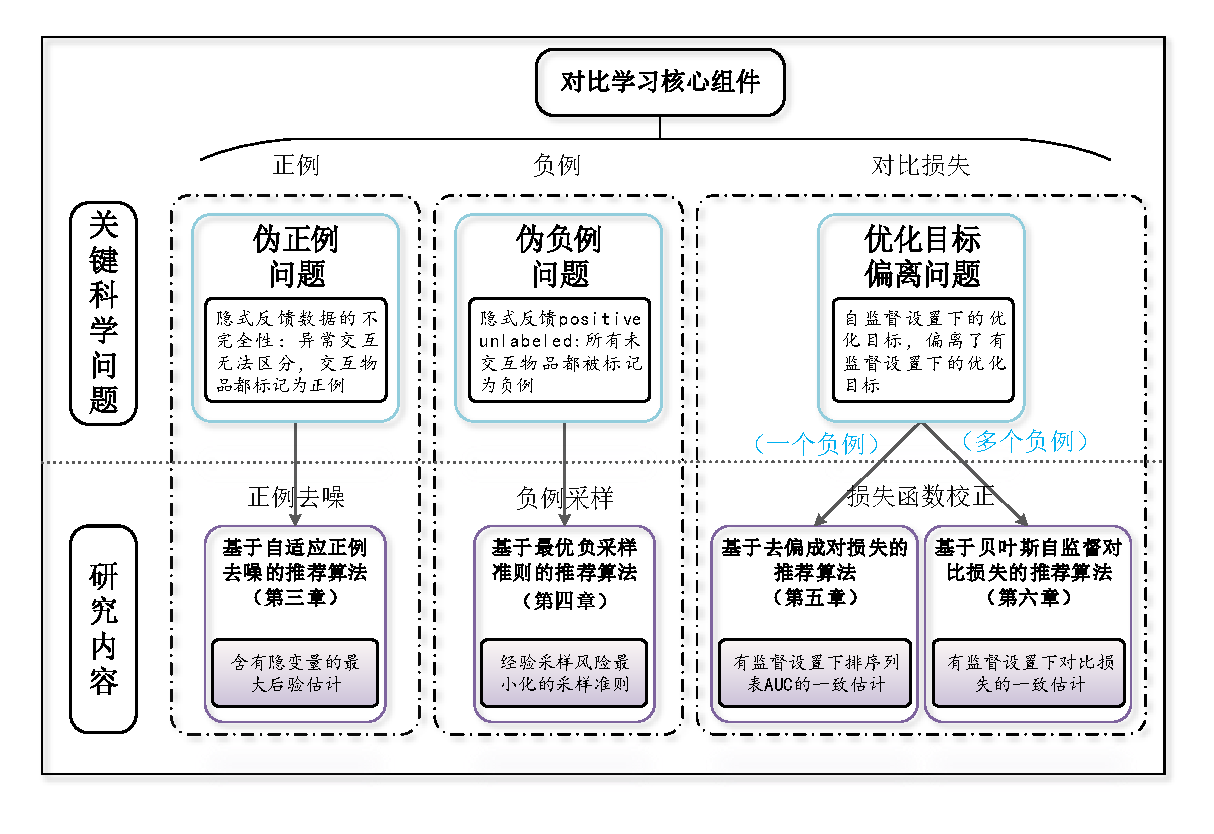
\includegraphics[width=\textwidth]{content.pdf}
	\caption{关键问题与研究内容的关系}
	\label{1Fig:content}
\end{figure*}
%*******************************

针对伪正样本问题,提出了自适应学习的成对排序算法,用于从含噪成对比较的数据中学习个性化排序。分析了隐式反馈的本质是数据不完全(incomplete data),并把从含噪成对比较的数据中学习排序的问题形式化为一个含有隐变量的最大后验估计问题。引入一个隐变量作为衡量交互置信度的新指标,这个隐变量与用户物品的特征表示一起作为模型参数一起端到端地学习。所提出的算法采用期望最大化框架:在期望步骤中使用贝叶斯推断来估计交互的置信度指标;在最大化步骤中固定置信度指标,更新参数学习用户和物品的特征表示。该算法在合成的噪声数据集上表现出了更好的鲁棒性,在真实的数据集上表现出更高的推荐准确性。

针对伪负样本问题,提出了贝叶斯最优负采样算法,用于从未标记的数据中采样高质量的负例,以提升对比学习的训练效果并提升推荐精度。提出了贝叶斯最优负采样准则,这是最小化经验采样风险的理论最优的采样规则。该方法指定了后验概率意义上的负信号测度,结合了静态的先验信息和动态的样本信息,统一了现有的两种提取负信号的两种主要范式,并为使用辅助信息建模先验概率的方法提供了灵活的接口。该算法在采样误差率和采样样本信息量以及推荐准确性上优于同类方法。

针对有偏的成对损失优化目标,提出了去偏成对学习算法,以近似完全监督数据的成对损失函数,以获得接近于有监督学习的泛化性能。该方法通过校正伪负样本导致的概率估计偏差,从而修正梯度以近似完全监督数据的梯度。所提出的目标函数易于实现,不需要额外的辅助信息进行监督,也不需要过多的存储和计算开销。在保持严格的相对于成对学习的线性时间复杂度情况下,去偏成对学习算法取得了更高的推荐准确性。

针对有偏的对比损失优化目标,提出了贝叶斯自监督对比学习算法,通过重要性权重来纠正从无标签数据中随机选择的负样本引入的偏差。从单个权重来看,该方法提供了样本是真负例的后验概率估计,可以灵活统一地执行硬负例挖掘和伪负例去偏任务这两个冲突任务。从损失函数的数值来看,该方法提供了有监督数据下对比损失的一致估计,从而提升下游任务的泛化性能。在数值实验、个性化推荐和图像分类等多个任务上验证了贝叶斯自监督对比学习算法的有效性。只需要简单地修改损失函数,而无需额外的存储和计算开销。



